% English translation of 《矿井水灾时巷道系统中的逃生规划》
% Compile with: latexmk -xelatex Escape_Planning_Mine_Flooding_EN.tex
\documentclass[12pt,a4paper]{article}

\usepackage[top=2.5cm,bottom=2.5cm,left=2.5cm,right=2.5cm]{geometry}
\usepackage{amsmath}
\usepackage{fontspec}
\usepackage{unicode-math}
% Times-style text and math (system STIX Two fonts), matching the Times New Roman of the original
\setmainfont{Times New Roman}
\setmathfont{STIX Two Math}
\setsansfont{Arial}
\setmonofont{lmmono10-regular}[Extension=.otf]
% CJK font only for the Chinese data-file / sheet names that must stay in the code
\newfontfamily\cjkfont{Songti SC}

\usepackage{graphicx}
\usepackage{booktabs,array}
\usepackage{tikz}
\usetikzlibrary{arrows.meta}
\usepackage{caption}
\captionsetup{labelsep=quad, font=small, labelfont=bf, textfont=bf}
\captionsetup[table]{labelsep=period, labelfont=rm, textfont=rm}
\usepackage{xcolor}
\usepackage{listings}
\usepackage{enumitem}
\usepackage{indentfirst}
\usepackage[hidelinks]{hyperref}

\linespread{1.25}
\hyphenation{Dijkstra}
\setlength{\parindent}{2em}

% ----- heading style (mirrors the Chinese CUMCM-style template) -----
\renewcommand{\thesection}{\arabic{section}.}
\renewcommand{\thesubsection}{\arabic{section}.\arabic{subsection}}
\renewcommand{\thesubsubsection}{\arabic{section}.\arabic{subsection}.\arabic{subsubsection}}
\makeatletter
\renewcommand{\section}{\@startsection{section}{1}{\z@}{2.5ex \@plus 1ex}{1.5ex}{\centering\Large\bfseries}}
\renewcommand{\subsection}{\@startsection{subsection}{2}{\z@}{2ex \@plus .5ex}{1ex}{\large\bfseries}}
\renewcommand{\subsubsection}{\@startsection{subsubsection}{3}{\z@}{1.5ex \@plus .5ex}{0.8ex}{\normalsize\bfseries}}
\renewcommand{\@seccntformat}[1]{\csname the#1\endcsname\quad}
\makeatother

% ----- code style -----
\definecolor{codebg}{gray}{0.96}
\lstset{
  basicstyle=\ttfamily\footnotesize,
  backgroundcolor=\color{codebg},
  keywordstyle=\color{blue!70!black},
  commentstyle=\color{green!40!black},
  stringstyle=\color{purple!70!black},
  breaklines=true, columns=fixed, keepspaces=true,
  showstringspaces=false, frame=none, xleftmargin=0pt,
  literate={³}{{$^3$}}1,
  escapechar=§,
}
\lstdefinestyle{py}{language=Python}
\lstdefinestyle{mat}{language=Matlab}

\newcommand{\appsection}[2]{%
  \section*{Appendix #1\quad #2}%
  \addcontentsline{toc}{section}{Appendix #1\quad #2}}

\begin{document}

% =====================================================================
\begin{center}
  {\LARGE\bfseries Escape Planning in Mine Tunnel Systems\\[2pt] during Mine Flooding}
\end{center}
\vspace{-0.3em}
\begin{center}
  {\Large\bfseries Abstract}
\end{center}
\vspace{-0.5em}
\begingroup\linespread{1.0}\selectfont
\enlargethispage{3\baselineskip}

Mine flooding is a major type of safety accident, and fast, accurate emergency decisions after a water inrush are the key to reducing casualties. The difficulty in making these decisions is that the spread of the floodwater and the escape of personnel are dynamically coupled in both time and space. The water flow changes the water-level environment, which in turn affects the escape routes, and the choice of route determines how long personnel are exposed to the hazardous environment. Tightly coupled through two globally shared variables---time and tunnel state---the tunnel network, the dynamics of the water flow, and the dynamic route planning of personnel together form an integrated system that reflects the interaction between the evolving disaster and emergency decision-making.

This paper builds a coupled modeling framework of ``water-flow simulation -- network construction -- route optimization''. For the water-spread model, our team represents the tunnel network as a graph constructed with a search algorithm. Based on the assumption that water first spreads while keeping the initial inflow height of 0.1\,m, and that any water above this level automatically flows into the branches, we establish a dynamic water-spread model. A priority-queue algorithm ensures that nodes reached earlier split their flow first, so that we can compute the key time series for every tunnel. For miner escape route planning, our team innovatively converts these time series into a dynamic network with time-varying weights. Following the relationships among walking speed, water depth and flow direction, we determine the speed in each situation and obtain the edge weights---the time needed to pass through a given tunnel---as functions of the time at which a miner passes through, establishing a coupled dynamic optimization model. To solve it, our team uses a time-dependent shortest-path algorithm based on Dijkstra's algorithm to find the time-optimal escape route for each miner.

For the data given in the attachments, our model successfully simulates the spread of water under single- and multiple-inrush scenarios, and obtains the optimal escape routes for miners at different locations and with different warning times. The simulation results show that when the tunnels lie in the same plane, the water spreads relatively widely; when the tunnels form a three-dimensional structure, elevation hinders the water from spreading upward, so the structure of the tunnel system and the location and elevation of the inrush point decisively shape the spread pattern. The route-planning results show that, based on each worker's location, we can plan the most suitable route to an exit and choose the exit that can be reached first. Moreover, as tunnels become flooded over time, early warning allows miners to detour at higher speed, and all routes eventually converge onto the main tunnel leading to the exit, which raises the chance of a successful escape. With multiple inrush sources, however, the plan needs to be adjusted in time.

The model has a concise physical mechanism, very high computational efficiency and broad applicability. Specific highlights include: when simulating the water spread, we treat the inrush point as a node, which improves both computational efficiency and clarity; in escape route planning, we use linear interpolation to make the assumption of a temporarily fixed initial water level continuous, which simplifies the complex, coupled water flow of reality while improving the model's agreement with reality. Overall, the model not only applies to the given scenarios, but can also provide a degree of quantitative decision support and theoretical backing for real-world emergency rescue in mine flooding.

\vspace{1em}
{\raggedright\noindent\textbf{\sffamily Keywords:}\quad Water spread;\ \ Tunnel system;\ \ Priority-queue algorithm;\ \ Escape planning;\ \ Dijkstra's algorithm\par}
\endgroup

\newpage
% =====================================================================
\renewcommand{\contentsname}{\centerline{Contents}}
\tableofcontents
\newpage

% =====================================================================
\section{Introduction}

As one of the five major natural hazards in China's coal mines, water hazards seriously constrain the healthy development of the coal industry, and their suddenness can easily cause heavy casualties and economic losses\textsuperscript{[1]}. Emergency strategies at the moment of a water inrush are therefore especially important. Water inrushes are sudden and random, difficult to detect in time, and change dynamically; the water spreads quickly, blocks the miners' escape and threatens their lives. Understanding the tunnel system and the direction in which the water spreads during an inrush, and then planning escape routes, can therefore reduce this major threat. The models below are built step by step following a logic that goes from simple to complex tunnel systems, from a single inrush point to multiple inrush points, and from analyzing the water spread to planning the escape, with the aim of offering a solution for mine flooding.

\section{Problem Restatement and Analysis}

This problem can be broken down into two major tasks: Problems 1 and 3 form Task 1, and Problems 2 and 4 form Task 2. Task 1 is to build water-spread models for different numbers of inrush points and use them for prediction. Specifically, we need to simulate the dynamic spread of water through a complex three-dimensional tunnel network under single-point and multi-point inrush scenarios, and compute the key time parameters of each tunnel, including the time at which the water arrives and the time at which the tunnel is completely filled. Task 2 is a dynamic optimization problem: planning dynamic escape routes for the miners. Using the direction and timing of the water flow obtained in the previous task, and taking into account how the water level constrains walking speed, we dynamically plan time-optimal escape routes for miners at specific locations in the disaster environment.

The complexity of the tunnel system shows in its large number of nodes; moreover, the tunnels do not connect every pair of neighboring nodes one by one, but connect them partially in a structured way. This means the modeling has to start from the tunnel containing the inrush point. Preliminary plots made in MATLAB revealed some complex structures in the tunnel system, such as loops and grids, which need extra attention when modeling the water flow: the fluid nature of the water has to be partly set aside, so that the water becomes a wall-hugging ``block'' of fixed height. At the same time, when the tunnels lie at different elevations, the water-flow model must be simplified and must include the fact that water cannot flow uphill because of elevation differences---this is a key difficulty in the modeling.

After the simplified water-flow simulation has been completed for Problems 1 and 3 as required, the second group of tasks asks us to optimize the personnel escape routes through dynamic scheduling, based on the flow conditions in the tunnel system. Once the problem is converted into minimizing the escape time, it can be viewed as a dynamic optimization problem. The key to solving it is to simulate the dynamic process in code and to use suitable algorithms to carry out the dynamic scheduling. Problem 4 adds a delayed second inrush point, which may require additional work in the code and is another difficulty in the modeling.

We summarize our analysis of the problems, the models we built, their roles and their relationships in the mind map in Figure~\ref{fig:mindmap}, shown below:

\begin{figure}[htbp]
  \centering
  \resizebox{\textwidth}{!}{% Figure 1 (redrawn in English from the original Chinese mind map)
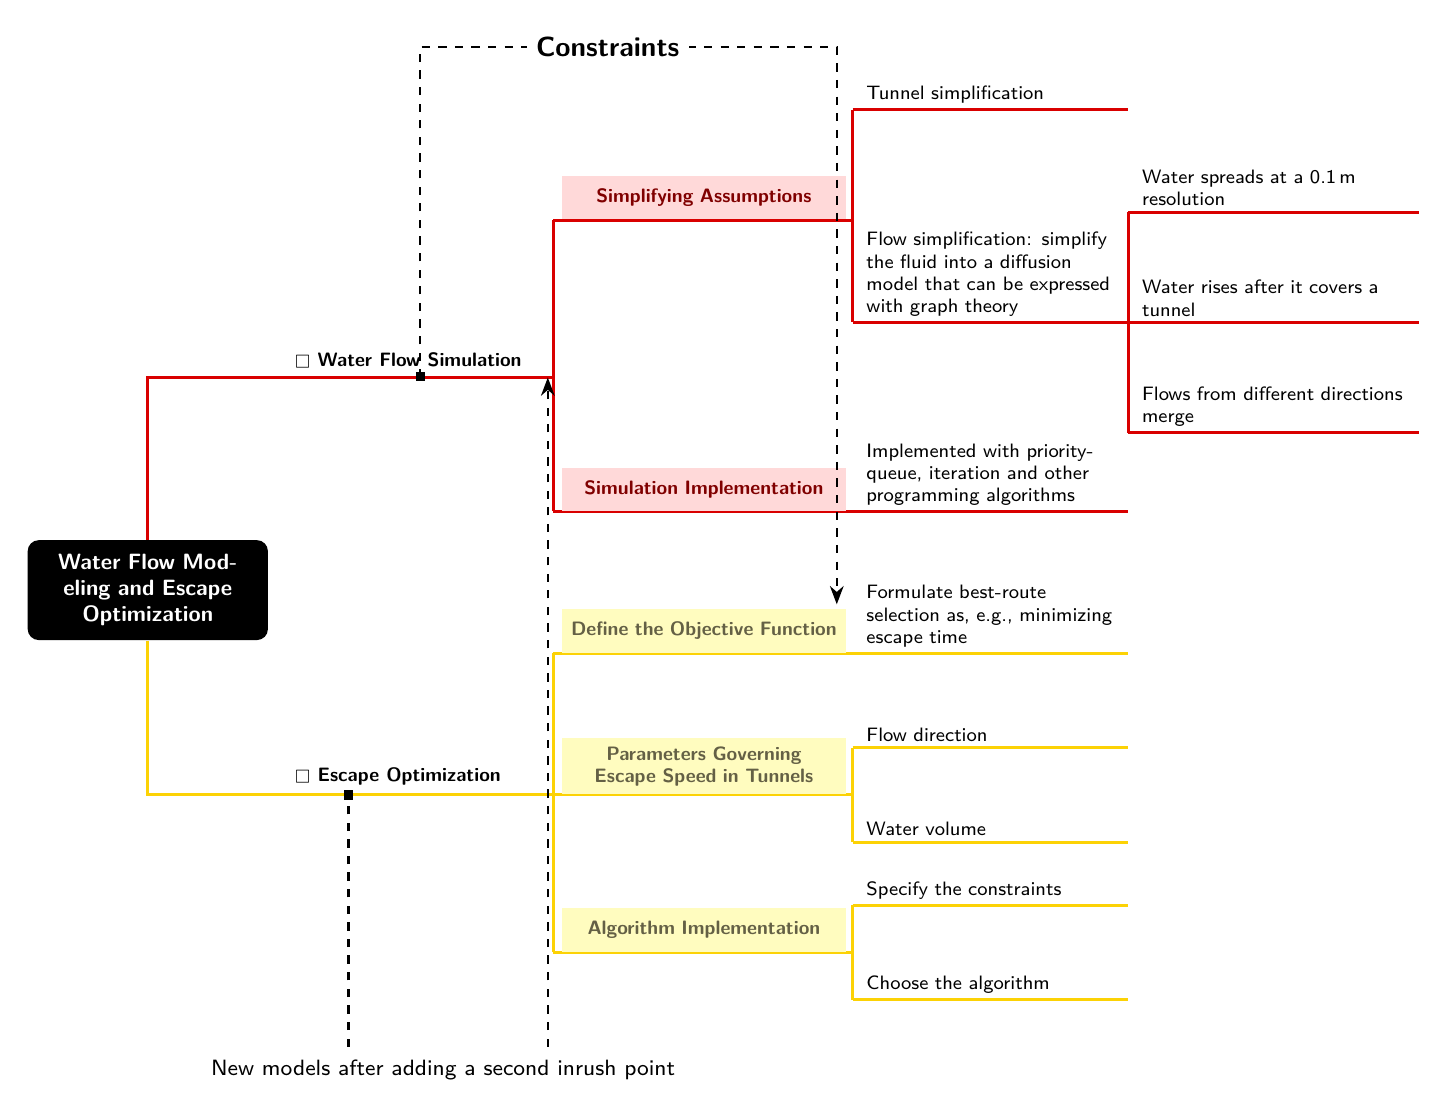
\begin{tikzpicture}[
    font={\sffamily\scriptsize\hyphenpenalty=10000},
    cat/.style={anchor=south west, text width=3.4cm, align=center, inner sep=3pt,
                minimum height=0.55cm, font={\sffamily\scriptsize\bfseries\hyphenpenalty=10000}},
    redcat/.style={cat, fill=red!15, text=red!50!black},
    yelcat/.style={cat, fill=yellow!25, text=yellow!30!black},
    leaf/.style={anchor=south west, align=left, text width=3.2cm, inner sep=2pt},
    sub/.style={anchor=south west, align=left, text width=3.4cm, inner sep=2pt},
    rline/.style={red!85!black, line width=1.1pt},
    yline/.style={yellow!70!orange, line width=1.1pt},
  ]
  % ---- root ----
  \node[fill=black, text=white, rounded corners=4pt, font=\sffamily\footnotesize\bfseries,
        align=center, text width=2.7cm, inner sep=5pt] (root) at (1.45,3.6)
        {Water Flow Modeling and Escape Optimization};

  % ---- red branch: water flow simulation ----
  \draw[rline] (root.north) |- (6.6,6.3);
  \node[anchor=south west, font=\sffamily\scriptsize\bfseries] at (3.2,6.3) {$\mdlgwhtsquare$ Water Flow Simulation};
  \draw[rline] (6.6,8.3) -- (6.6,4.6);
  % Simplifying assumptions
  \draw[rline] (6.6,8.3) -- (10.4,8.3);
  \node[redcat] at (6.7,8.3) {Simplifying Assumptions};
  \draw[rline] (10.4,9.7) -- (10.4,7.0);
  \draw[rline] (10.4,9.7) -- (13.9,9.7); \node[leaf] at (10.5,9.7) {Tunnel simplification};
  \draw[rline] (10.4,7.0) -- (13.9,7.0); \node[leaf] at (10.5,7.0) {Flow simplification: simplify the fluid into a diffusion model that can be expressed with graph theory};
  \draw[rline] (13.9,8.4) -- (13.9,5.6);
  \draw[rline] (13.9,8.4) -- (17.6,8.4); \node[sub] at (14.0,8.4) {Water spreads at a 0.1\,m resolution};
  \draw[rline] (13.9,7.0) -- (17.6,7.0); \node[sub] at (14.0,7.0) {Water rises after it covers a tunnel};
  \draw[rline] (13.9,5.6) -- (17.6,5.6); \node[sub] at (14.0,5.6) {Flows from different directions merge};
  % Simulation implementation
  \draw[rline] (6.6,4.6) -- (13.9,4.6);
  \node[redcat] at (6.7,4.6) {Simulation Implementation};
  \node[leaf] at (10.5,4.6) {Implemented with priority-queue, iteration and other programming algorithms};

  % ---- yellow branch: escape optimization ----
  \draw[yline] (root.south) |- (10.4,1.0);
  \node[anchor=south west, font=\sffamily\scriptsize\bfseries] at (3.2,1.0) {$\mdlgwhtsquare$ Escape Optimization};
  \draw[yline] (6.6,2.8) -- (6.6,-1.0);
  % Objective
  \draw[yline] (6.6,2.8) -- (13.9,2.8);
  \node[yelcat] at (6.7,2.8) {Define the Objective Function};
  \node[leaf] at (10.5,2.8) {Formulate best-route selection as, e.g., minimizing escape time};
  % Parameters
  \node[yelcat] at (6.7,1.0) {Parameters Governing Escape Speed in Tunnels};
  \draw[yline] (10.4,1.6) -- (10.4,0.4);
  \draw[yline] (10.4,1.6) -- (13.9,1.6); \node[leaf] at (10.5,1.6) {Flow direction};
  \draw[yline] (10.4,0.4) -- (13.9,0.4); \node[leaf] at (10.5,0.4) {Water volume};
  % Algorithm
  \draw[yline] (6.6,-1.0) -- (10.4,-1.0);
  \node[yelcat] at (6.7,-1.0) {Algorithm Implementation};
  \draw[yline] (10.4,-0.4) -- (10.4,-1.6);
  \draw[yline] (10.4,-0.4) -- (13.9,-0.4); \node[leaf] at (10.5,-0.4) {Specify the constraints};
  \draw[yline] (10.4,-1.6) -- (13.9,-1.6); \node[leaf] at (10.5,-1.6) {Choose the algorithm};

  % ---- dashed relations ----
  \fill (4.85,6.25) rectangle ++(0.12,0.12);
  \draw[dashed, thick, -{Stealth}] (4.91,6.3) -- (4.91,10.5) -- (10.2,10.5)
        node[pos=0.45, fill=white, font=\sffamily\bfseries\normalsize] {Constraints} -- (10.2,3.42);
  \node[font=\sffamily\footnotesize] at (5.2,-2.5) {New models after adding a second inrush point};
  \draw[dashed, thick] (4.0,-2.2) -- (4.0,1.0);
  \fill (3.94,0.94) rectangle ++(0.12,0.12);
  \draw[dashed, thick, -{Stealth}] (6.53,-2.2) -- (6.53,6.3);
\end{tikzpicture}
}
  \caption{Problem analysis roadmap}
  \label{fig:mindmap}
\end{figure}

\section{Model Assumptions}

Our team made strong simplifications of the water-spread process after the inrush, and made the following assumptions accordingly:
\begin{itemize}[leftmargin=2em]
  \item After passing through a node, the inrush water keeps the same height and divides its flow rate equally among the other tunnels connected to that node.
  \item Water flows through a tunnel at a uniform speed, in a straight line along the tunnel.
  \item On a very small time scale, the inrush water enters a tunnel and begins to spread at a height of 0.1\,m. We assume it keeps spreading in this way until all tunnels are covered by water 0.1\,m high; during this stage, when the water splits at tunnel nodes it keeps a height of 0.1\,m, while its flow rate is divided equally according to the number of branch tunnels connected to the node.
  \item Once all tunnels are covered by water, i.e., once the water level everywhere reaches 0.1\,m, the water preferentially flows into tunnels (and their branches) that have not yet been filled; flow is no longer sent into tunnels that are already filled, but is transferred entirely to tunnels that are not yet filled.
\end{itemize}

\section{Notation}

\begin{table}[htbp]
  \centering
  \renewcommand{\arraystretch}{1.15}
  \begin{tabular}{>{\centering\arraybackslash}p{2.6cm} >{\centering\arraybackslash}p{12.4cm}}
    \toprule
    Symbol & Meaning \\
    \midrule
    $P$ & Set of node coordinates \\
    $H$ & Set of tunnel edges \\
    $e_{ij}$ & An element of the edge set $H$; $i$ and $j$ are the two nodes of edge $e$, which together identify a specific tunnel \\
    $L_{e_{ij}}$ & Length of each tunnel \\
    $t_{arrival}(e_{ij})$ & Time at which the spreading water reaches each tunnel \\
    $t_{full}(e_{ij})$ & Time at which the spreading water fills each tunnel \\
    $V_{water}(e_{ij})$ & Flow rate (volume per unit time) of the spreading water in each tunnel \\
    $V_{ij}$ & Miner's escape speed \\
    $h$ & Water depth in a tunnel \\
    $t_{ij}$ & Miner's escape time between nodes $i$ and $j$ (i.e., to traverse $e_{ij}$) \\
    $T_{total}$ & Total time a miner needs to escape \\
    $d$ & Miner's direction relative to the water flow in a tunnel, i.e., upstream or downstream \\
    $Path$ & Set of nodes passed through in a miner's escape route plan \\
    $F$ & Outflow rate of any tunnel over a given (almost instantaneous) time interval \\
    $\widetilde{F}$ & Inflow rate of any tunnel over a given (almost instantaneous) time interval \\
    \bottomrule
  \end{tabular}
\end{table}

\section{Model Building and Solution}

We drew the modeling framework together with the algorithms used by each model, to show more clearly the inputs and outputs and how they relate to each other.

\begin{figure}[htbp]
  \centering
  \resizebox{\textwidth}{!}{% Figure 2 (redrawn in English from the original Chinese flowchart)
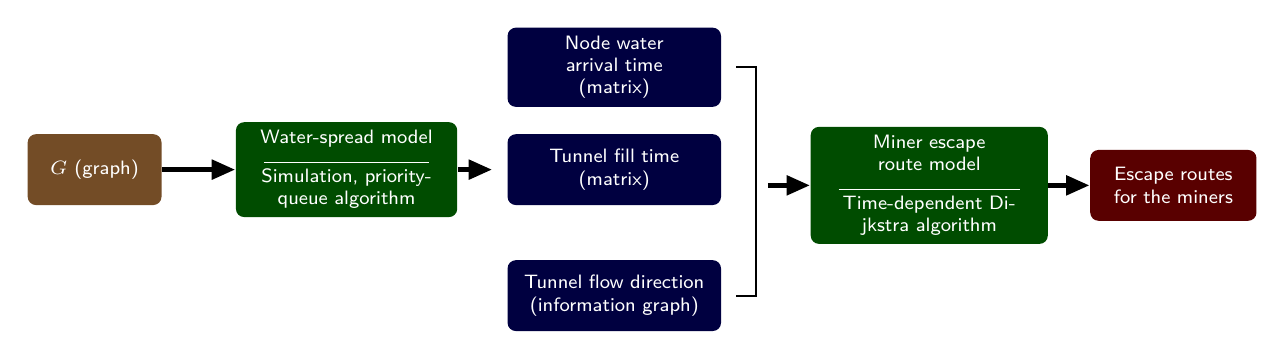
\begin{tikzpicture}[
    font=\sffamily\scriptsize,
    box/.style={rounded corners=3pt, text=white, align=center, minimum height=0.9cm, inner sep=3pt},
    arr/.style={-{Triangle[length=3mm,width=2.4mm]}, line width=2pt},
  ]
  \node[box, fill=brown!60!black, minimum width=1.7cm] (G) at (0,0) {$G$ (graph)};
  \node[box, fill=green!30!black, text width=2.6cm] (W) at (3.2,0)
       {Water-spread model\\[-1pt]\rule{2.1cm}{0.3pt}\\[-1pt]Simulation, priority-queue algorithm};
  \node[box, fill=blue!25!black, text width=2.5cm] (A) at (6.6,1.3) {Node water arrival time\\(matrix)};
  \node[box, fill=blue!25!black, text width=2.5cm] (F) at (6.6,0.0) {Tunnel fill time\\(matrix)};
  \node[box, fill=blue!25!black, text width=2.5cm] (D) at (6.6,-1.6) {Tunnel flow direction\\(information graph)};
  \node[box, fill=green!30!black, text width=2.8cm] (M) at (10.6,-0.2)
       {Miner escape route model\\[-1pt]\rule{2.3cm}{0.3pt}\\[-1pt]Time-dependent Dijkstra algorithm};
  \node[box, fill=red!35!black, text width=1.9cm] (R) at (13.7,-0.2) {Escape routes for the miners};
  \draw[arr] (G) -- (W);
  \draw[arr] (W) -- (5.05,0);
  \draw[thick] (8.15,1.3) -- (8.4,1.3) -- (8.4,-1.6) -- (8.15,-1.6);
  \draw[arr] (8.55,-0.2) -- (M);
  \draw[arr] (M) -- (R);
\end{tikzpicture}
}
  \caption{Modeling and solution framework}
  \label{fig:framework}
\end{figure}

\subsection{Problem 1}

\subsubsection{Data Preprocessing}

To determine the location of the inrush point and the structure of the tunnel system, our team first plotted the data given in Attachments 1 and 2. By looking at the 3D plots, we gained a general understanding of the tunnel layout and how water might spread. The red dot is the inrush point, blue dots are nodes, and gray lines are tunnels. To show the tunnel system more clearly, the height (i.e., the $z$-axis) was exaggerated by a factor of 100 when plotting. The resulting plots are shown below:

\begin{figure}[htbp]
  \centering
  \begin{minipage}{0.48\textwidth}
    \centering
    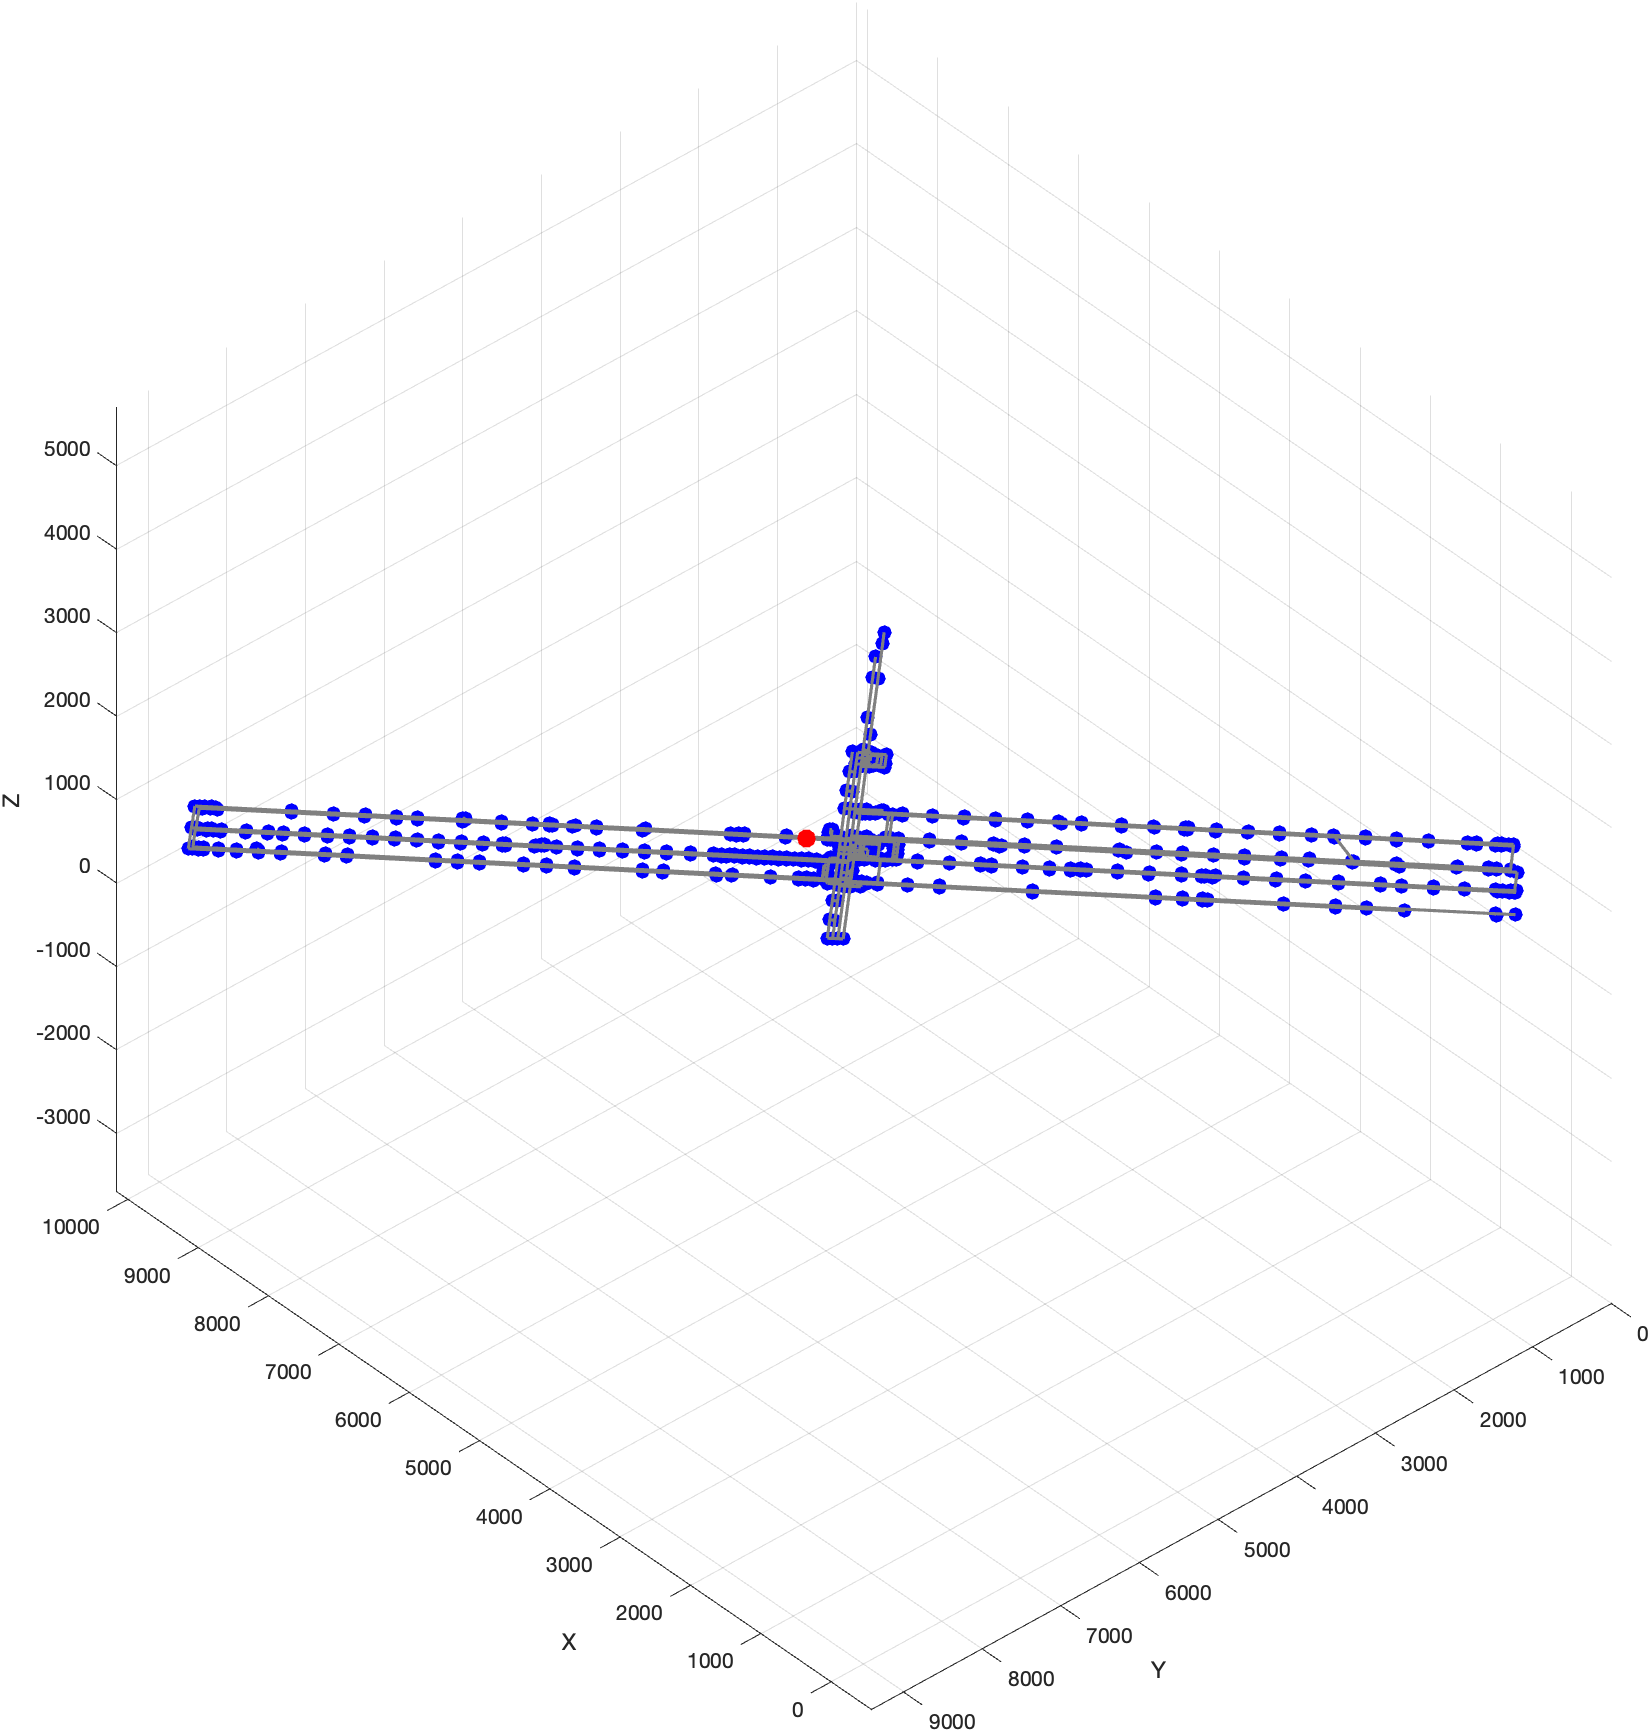
\includegraphics[width=\linewidth]{figures/fig03_att1_3d.png}
    \caption{3D view of the tunnel system in Attachment 1}
    \label{fig:att1-3d}
  \end{minipage}\hfill
  \begin{minipage}{0.48\textwidth}
    \centering
    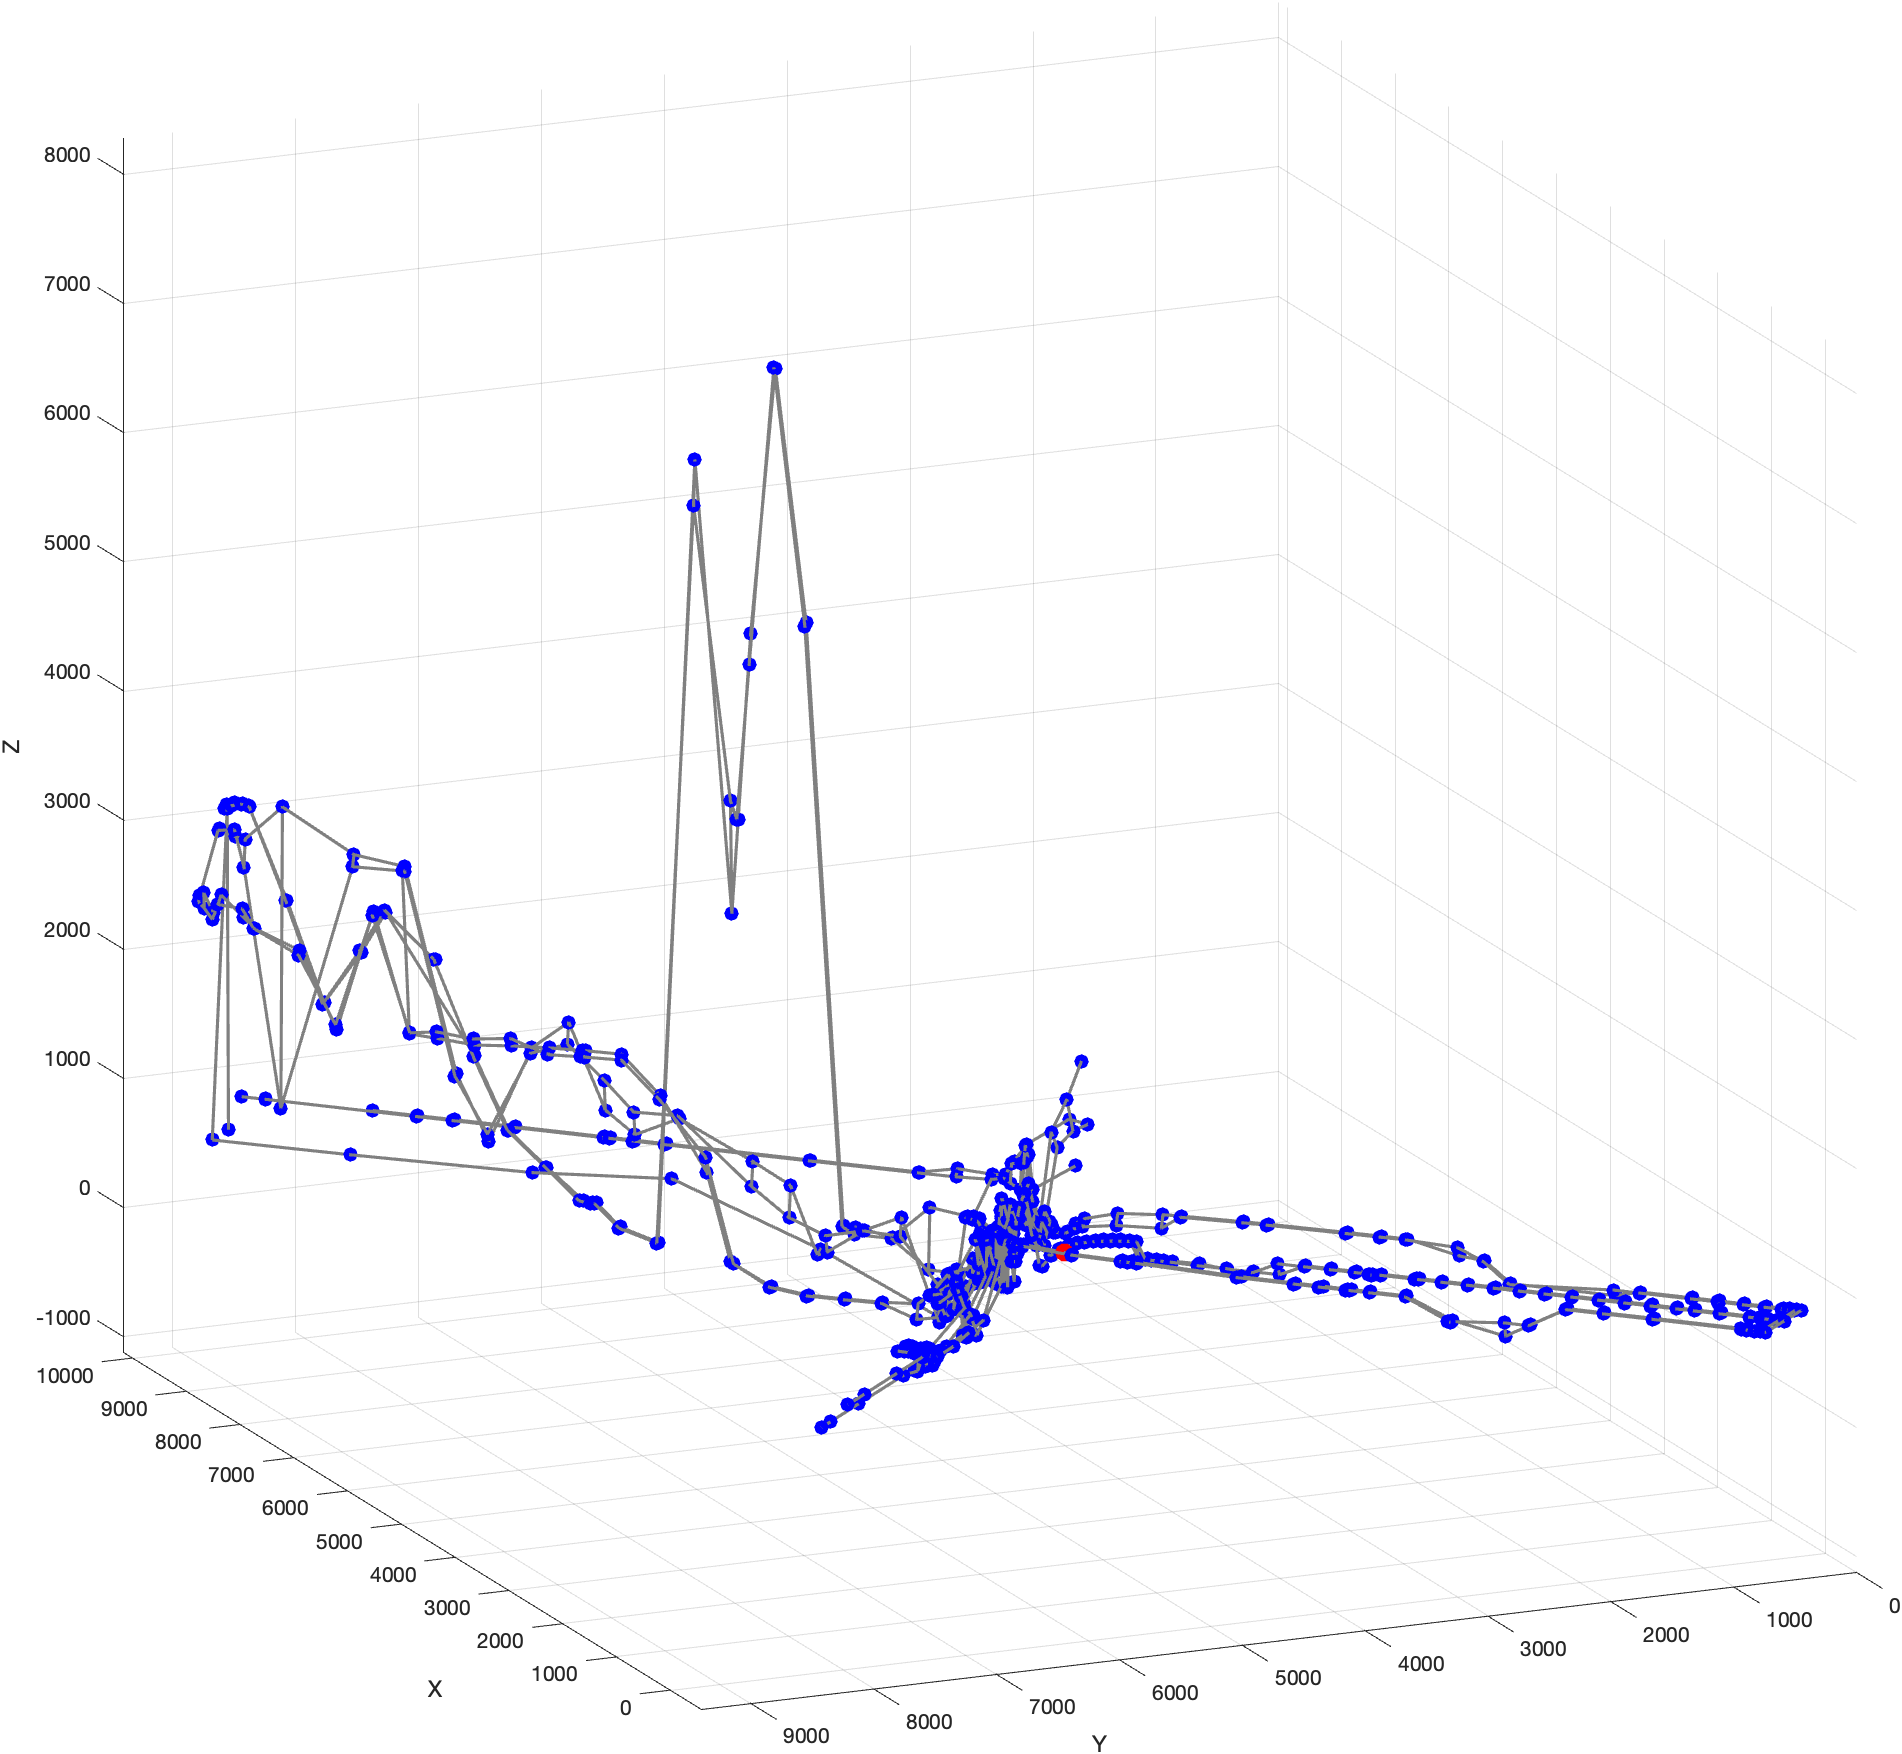
\includegraphics[width=\linewidth]{figures/fig04_att2_3d.png}
    \caption{3D view of the tunnel system in Attachment 2}
    \label{fig:att2-3d}
  \end{minipage}
\end{figure}

\subsubsection{Problem Analysis}

For Attachment 1, since all parts of the tunnel system have the same height (i.e., all nodes have the same $z$-coordinate), the tunnel system lies in a single plane. Following the basic assumptions above, we let the water spread while keeping a height of 0.1\,m. Since this problem is purely computational, our team completed it by programming in Python. We search the file for the tunnels connected to the inrush point, and, based on the assumption of a fixed initial water height, abstract the water flow as a model that expands through the graph. After a tunnel is covered, its water level rises according to the flow rate at the node until it reaches the tunnel height of 3\,m, after which the entire flow is divided equally and transferred to other tunnels; this continues until all tunnels are filled with water.

For Attachment 2, the tunnel system adds a height attribute: unlike Attachment 1, where all tunnels are at the same level, the system in Attachment 2 contains both inclined and horizontal tunnels, and the inclined tunnels all have different angles of inclination, as shown in Figure~\ref{fig:att2-3d}. We still keep the basic assumptions from the previous part, with water flowing along the floor of each tunnel at a height of 0.1\,m, and analyze on that basis. It is worth noting that this problem adds the constraint that water cannot flow up inclined tunnels; this part is implemented additionally in code, again in Python.

In addition, our team plotted the number of branches at each node to observe how complex the system is. The figures below show, for Attachments 1 and 2 respectively, how many nodes have each number of branches; the horizontal axis is the number of branches at a node, and the vertical axis is the number of nodes with that number of branches:

\begin{figure}[htbp]
  \centering
  \begin{minipage}{0.48\textwidth}
    \centering
    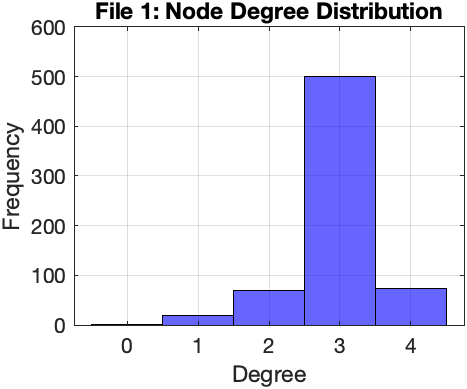
\includegraphics[width=0.8\linewidth]{figures/fig05_att1_degree.png}
    \caption{Number of branches per node, Attachment 1}
  \end{minipage}\hfill
  \begin{minipage}{0.48\textwidth}
    \centering
    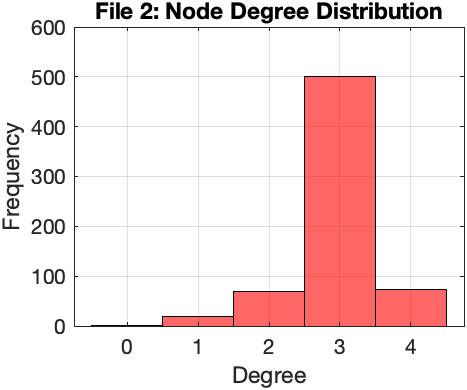
\includegraphics[width=0.8\linewidth]{figures/fig06_att2_degree.png}
    \caption{Number of branches per node, Attachment 2}
  \end{minipage}
\end{figure}

What the two tunnel systems have in common is that the number of nodes with 3 branches is especially high, making up the large majority of all nodes (about $\frac{3}{4}$ of the total), followed by nodes with 2 and 4 branches, which shows that the systems are fairly complex. In addition, the branch-count statistics in the two figures are exactly the same, which may be because the tunnel layout in Attachment 2 is a rotation of the structure in Attachment 1.

As for how water accumulates: once the front of the water reaches the end of a tunnel, the tunnel begins to fill, and from then on the water level in the tunnel keeps rising. The law $h(e,t)$ describing how the height changes with time $t$ is derived from a volume balance for the tunnel. $\widetilde{F}$ is the inflow rate during this period and $F$ is the outflow rate during this period.

Specifically, the stored volume is first:
\begin{equation}
  Q(h) = 4\cdot L_e \cdot h
\end{equation}
and we also have:
\begin{equation}
  \frac{dQ}{dt} = \widetilde{F} - F
\end{equation}

We built this model to describe the flow process in a tunnel whose water level is above the initial inrush level that covers the tunnels (0.1\,m) but has not yet reached the full level (3\,m). While a tunnel is filling in this way, its outlet end can be regarded as closed, so the outflow $F$ from the tunnel is 0. The rate at which the water level rises then becomes:
\begin{equation}
  \frac{dh}{dt} = \frac{\widetilde{F}}{4\cdot L_e}
\end{equation}

Rearranging the equation above gives the time needed to fill the tunnel, where the height difference is the difference between the full level (3\,m) and the current level (0.1\,m). The relationship between the water arrival time $t_{arrival}$ and the tunnel fill time $t_{full}$ is finally:
\begin{equation}
  t_{full} = t_{arrival} + \frac{(3-0.1)\cdot 4\cdot L_e}{\widetilde{F}} = t_{arrival} + \frac{11.6\cdot L_e}{\widetilde{F}}
\end{equation}

In summary, as required, solving this in code gives the time at which the water reaches each node and the time at which each tunnel is flooded to a height of 3\,m, which completes the modeling for this problem.

\subsubsection{Solution Approach}

The approaches for the two attachments are similar. The part implemented in code is as follows. We search the file for the tunnels connected to the inrush point, and, in the second sheet of the attachment, search from each node for the nodes connected to it to identify the tunnels and build the graph. Based on the assumption of a fixed initial water height, the water flow is abstracted as a model that expands through the graph; after a tunnel is covered, its water level rises according to the flow rate at the node until it reaches the tunnel height of 3\,m, after which the entire flow is divided equally and transferred to other tunnels, until all tunnels are filled with water. For the requirement in Attachment 2 that water cannot flow uphill, when searching for the nodes connected to a node we exclude tunnels that lead to nodes higher than the current node, so that each node only keeps paths that are no higher than itself; this gives a reasonable solution for the water-flow graph.

It is worth mentioning that a highlight of our solution is that, once the program finds the inrush point, it splits the tunnel containing the inrush point into two, treats the inrush point as a node and continues the computation, so the inrush point does not need to be treated separately as a source flowing toward both sides. This turns the inrush situation into an ordinary node-splitting situation, making the whole solution more convenient and elegant.

\subsubsection{Results}

Using a priority-queue algorithm\textsuperscript{[2]} to simulate the water flow in the tunnel system, we obtained the times at which water reaches the key nodes and the times at which the tunnels are filled. We plotted the trends of the node arrival times and tunnel fill times for Attachments 1 and 2 to observe how the water spreads through the whole tunnel system over time. The analysis of the key node and tunnel data shows that all of the water spread follows a roughly exponential rising trend. This means the water spreads relatively slowly at the beginning, so miners should be urged at this stage to head for an exit in the fastest way possible, even if the route is somewhat longer. As the water spreads faster over time, more attention should be paid to how the water height changes the workers' speed, and the flooding of tunnels should be checked, so that more reasonable routes can be found. The four figures below show the analysis of the key data for Problem 1. The complete results are in the result files produced by the code in Appendices A and B.

\begin{figure}[htbp]
  \centering
  \begin{minipage}{0.48\textwidth}
    \centering
    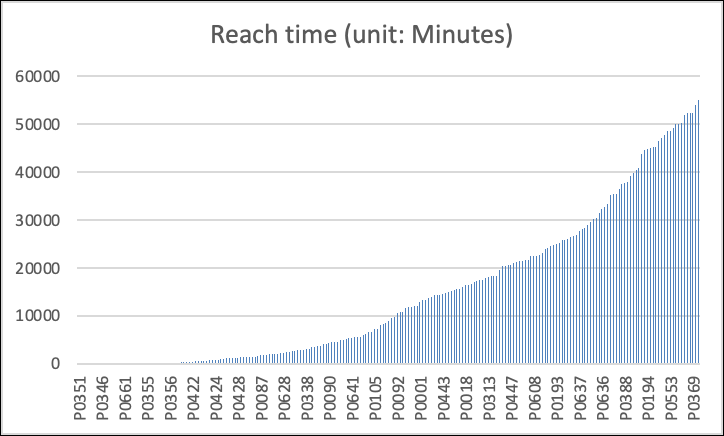
\includegraphics[width=\linewidth]{figures/fig07_att1_reach.png}
    \caption{Trend of water arrival times at nodes, Attachment 1}
  \end{minipage}\hfill
  \begin{minipage}{0.48\textwidth}
    \centering
    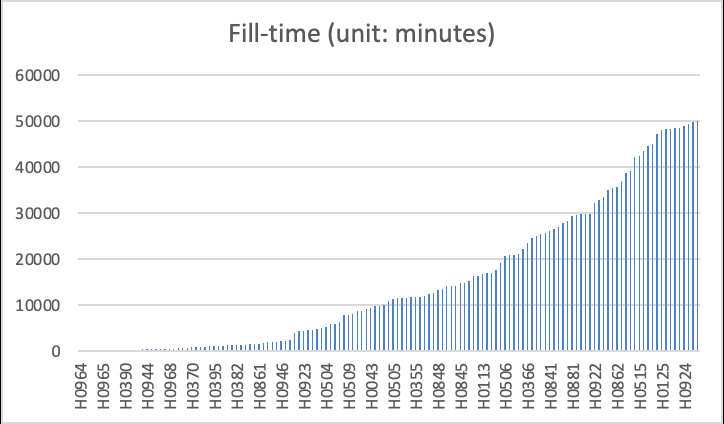
\includegraphics[width=\linewidth]{figures/fig08_att1_fill.png}
    \caption{Trend of tunnel fill times, Attachment 1}
  \end{minipage}\\[1em]
  \begin{minipage}{0.48\textwidth}
    \centering
    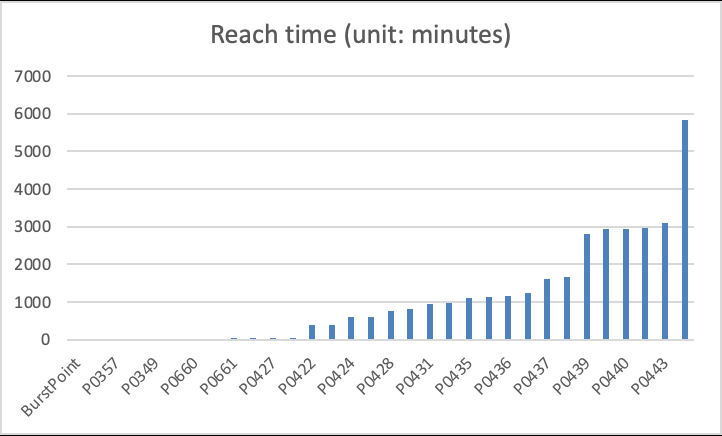
\includegraphics[width=\linewidth]{figures/fig09_att2_reach.png}
    \caption{Trend of water arrival times at nodes, Attachment 2}
  \end{minipage}\hfill
  \begin{minipage}{0.48\textwidth}
    \centering
    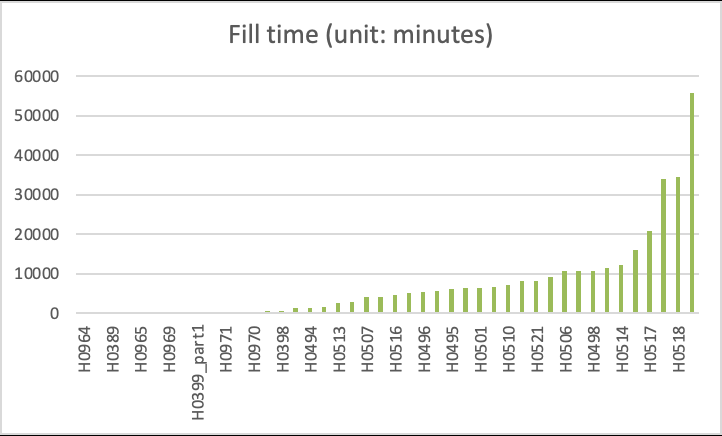
\includegraphics[width=\linewidth]{figures/fig10_att2_fill.png}
    \caption{Trend of tunnel fill times, Attachment 2}
  \end{minipage}
\end{figure}

\subsection{Problem 2}

\subsubsection{Problem Analysis}

This is an optimization problem with dynamic constraints. To plan the optimal escape route for a miner, the objective is to minimize the time $T_{total}$ the miner needs to get from their location to an exit, which requires considering both geometric distance and the effect of the water dynamics on the miner. Based on our analysis of the problem, our team worked out how each factor acts. The optimal escape route depends on the miner's speed $V$, the miner's speed depends directly on the water depth $h$, and the water depth in any tunnel depends on time. At the same time, optimal escape planning has to take each miner's location into account: the relationship between their different locations and the inrush point determines how strongly they are affected by the spreading water, so each escape plan is more individualized.

\subsubsection{Model Building}

We need to plan the miners' escape routes, so our team represents the final route plan as a set of nodes, $Path$; each node in the set is a point the miner will walk through. The first and last elements of the set correspond to the miner's initial position given in the problem, $(x_{start}, y_{start}, z_{start})$, and the position of one of the two exits, $(x_{final}, y_{final}, z_{final})$, respectively:
\begin{equation}
  Path = \{(x_{start}, y_{start}, z_{start}), (x_1, y_1, z_1), (x_2, y_2, z_2), \ldots, (x_{final}, y_{final}, z_{final})\}
\end{equation}

The route can also be expressed in terms of tunnel edges. In this case, the subscripts of the edges in the route set must link up end to end, so that the miner's escape route is continuous:
\begin{equation}
  Path = \{e_{ij}, e_{jk}, e_{kl}, \ldots, e_{pq}\}
\end{equation}

Our team treats the miner's speed as a piecewise function, and the traversal time as a dynamic variable that is determined by the water depth. As for the miner's direction of travel, this is exactly what we need to optimize. From Problem 1 we know the direction of the water flow, so we can tell whether the miner is moving with or against the flow. We define the tunnel network as a graph $G(P,H)$ consisting of the node set $P$ and the edge set $H$. For any edge $e_{ij}$ connecting nodes $i$ and $j$, its physical length is denoted $L_e$. The miner's speed on edge $e$ is defined as $V$, a function of the water depth $h$ and of the direction of travel $d$ relative to the flow. The speed $V$ (m/s) is then:
\begin{equation}
  V = \begin{cases}
    4 & \text{for } h = 0\\
    2 & \text{for downstream travel and } 0 < h \le 0.3\\
    1 & \text{for upstream travel and } 0 < h \le 0.3\\
    0 & \text{for } h > 0.3
  \end{cases}
\end{equation}
When $V=0$, the route is impassable.

The water depth $h$ is a piecewise function of the tunnel and of time: before the water reaches the tunnel, and after the tunnel is full, the water depth is constant. While water is entering the tunnel, the depth is a continuous function of time. The water depth function $h(e,t)$ is given below. The water arrival time $t_{arrival}(e)$ and fill time $t_{full}(e)$ of each tunnel are the results computed in Problem 1, and the flow rate $V_{water}(e)$ was also computed above, so all of them are known in this problem:
\begin{equation}
  h = \begin{cases}
    0 & t < t_{arrival}\\[2pt]
    0.1 + \dfrac{(t - t_{arrival})\cdot V_{water}(e)}{4\cdot L_e} & t_{arrival} \le t < t_{full}\\[8pt]
    3 & t \ge t_{full}
  \end{cases}
\end{equation}

From the speed and water depth above, the time to traverse tunnel edge $e$ is:
\begin{equation}
  t_{ij} = \frac{L_e}{V_{ij}}
\end{equation}

From this we can write the objective function, which sums the times and minimizes the total, where $t_{ij}$ is the time each miner spends in each tunnel:
\begin{equation}
  \min\quad T_{total} = \sum_{e_{ij}\in Path} t_{ij}
\end{equation}

In addition, the model must satisfy the following constraints:

\noindent Constraint 1 (a tunnel on the route must not already be filled with water):
\begin{equation}
  \forall e_{ij} \in Path,\quad V_{ij} > 0
\end{equation}
Constraint 2 (the tunnels on the escape route must exist):
\begin{equation}
  \forall\, i, j \text{ adjacent in } Path,\quad e_{ij} \in H
\end{equation}

\subsubsection{Solution Approach}

The code for Problem 2 uses the graph and the water-flow simulation obtained in Problem 1, which give two vectors: the times at which water reaches the tunnel nodes and the times at which the tunnels are flooded. Combining this information with an extra check on directions in the undirected graph, we can determine the specific value of the multivariable speed function $V(h(e,t), d)$. Using the Dijkstra-type algorithm\textsuperscript{[3]} built in the code, we can find the best routes for the three workers to get out of the tunnel system.

Concretely, our team's program reads the data and applies the alert delay, then determines the direction of the water flow and finds the neighboring nodes of each node; it then organizes this node information and uses Dijkstra's algorithm on the neighboring nodes to find the shortest route in real time. A highlight of our solution to this problem is the following: because speed and water level are so closely related in the time calculation, a good, reasonably continuous water-level model is needed. Starting from the results of the previous model, we use linear interpolation, which in a sense expands the data, to obtain the water level in each tunnel at every moment; this makes the water height continuous and convenient for route planning. Note that workers are assumed to stay still and do nothing else before they receive the inrush alert, and to start escaping along the planned route after one minute.

\subsubsection{Results}

\begin{figure}[htbp]
  \centering
  \begin{minipage}{0.48\textwidth}
    \centering
    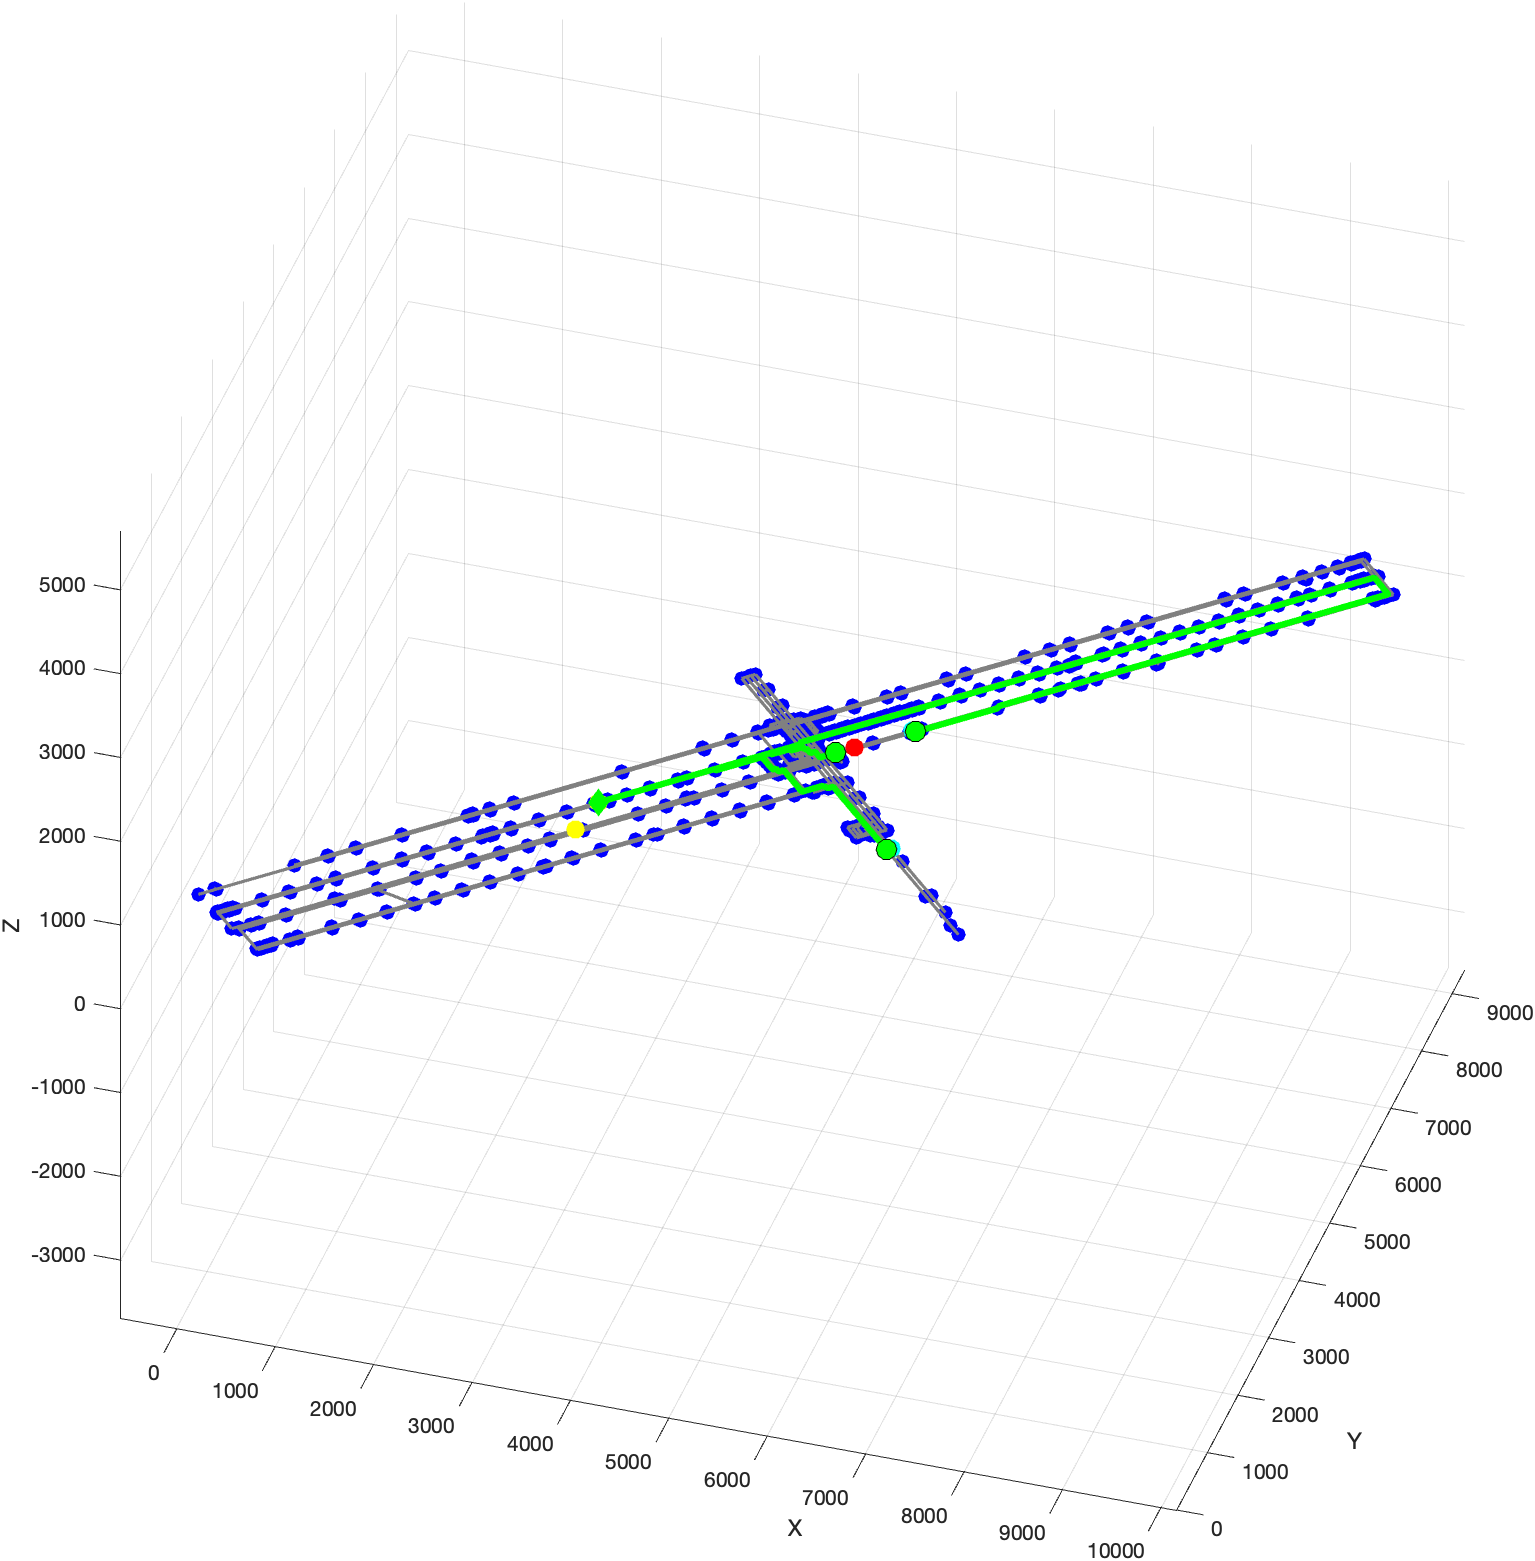
\includegraphics[width=\linewidth]{figures/fig11_att1_paths.png}
    \caption{Miner escape routes, Attachment 1}
    \label{fig:att1-paths}
  \end{minipage}\hfill
  \begin{minipage}{0.48\textwidth}
    \centering
    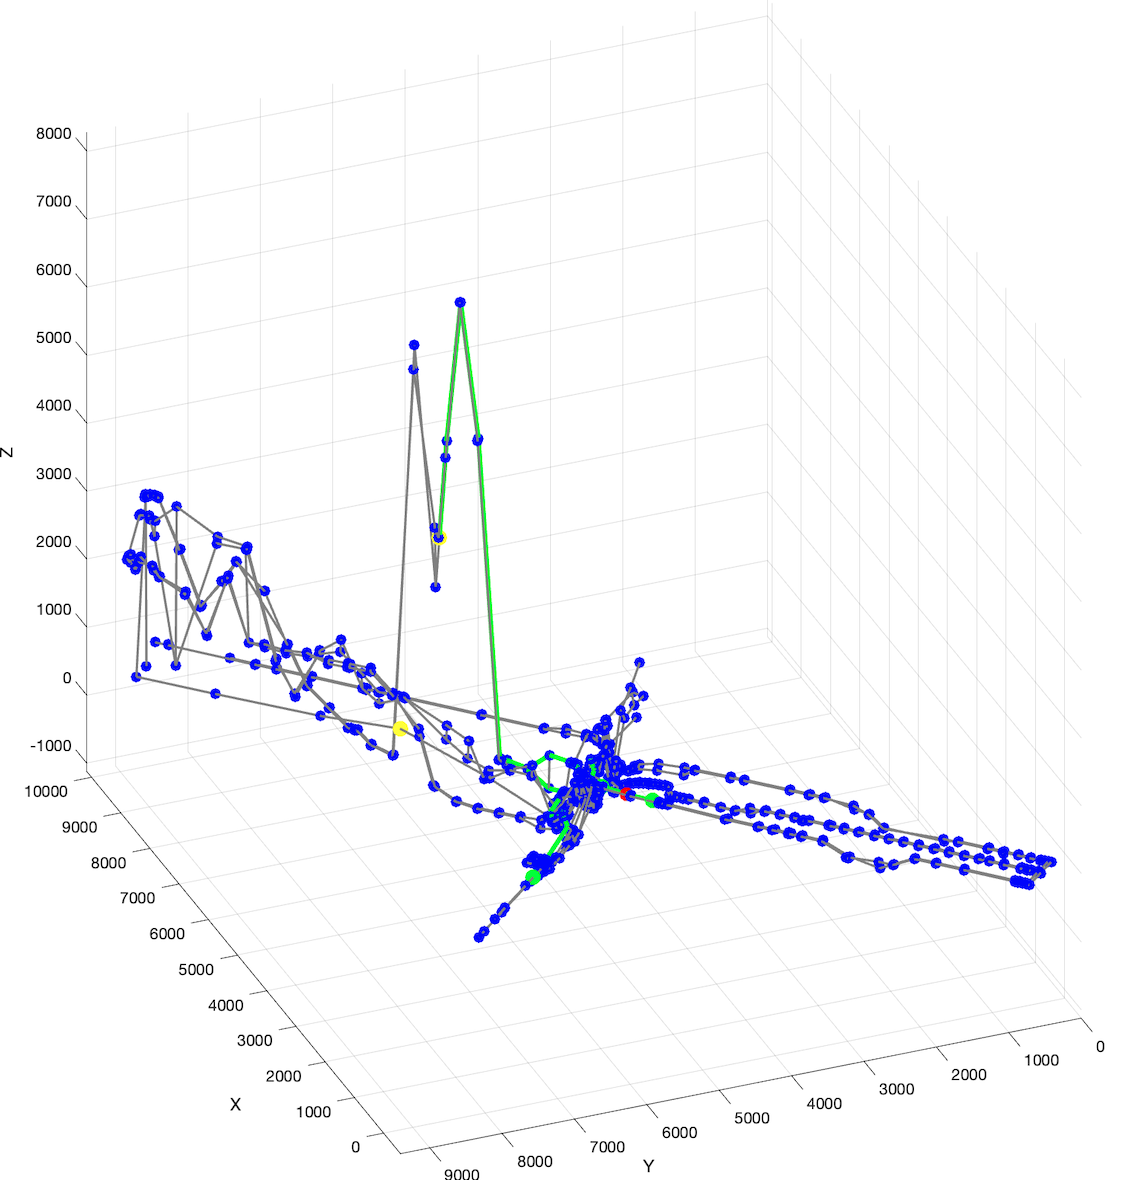
\includegraphics[width=\linewidth]{figures/fig12_att2_paths.png}
    \caption{Miner escape routes, Attachment 2}
    \label{fig:att2-paths}
  \end{minipage}
\end{figure}

For Attachment 1 in this problem, we used Dijkstra's algorithm to solve for the miners' escape routes and drew the escape route diagram in Figure~\ref{fig:att1-paths}. The red dot is the inrush point, the yellow dot and the green diamond are the exits, and the three green dots are the starting points of the three miners. All of the miners leave through the exit marked by the green diamond, going around the tunnels that are flooded early, especially those near the inrush point. The two miners closer to the inrush point both tend to leave the area around the inrush point first, even at the cost of a slightly longer detour. Although we want the optimal route to be as short as possible, the effect of the water on walking speed can lead to detours. This supports the reasonableness of the routes found by our model. Next, the figure shows that the tunnels leading to the green-diamond exit form a straight passage, and all miners gradually reach this passage and follow it to the exit. This tells us that this tunnel is the ``critical path'' of the system. In addition, the optimal escape routes show that the solutions do their best to avoid highly complex nodes.

For Attachment 2 in this problem, as shown in Figure~\ref{fig:att2-paths}, the two yellow dots are the exits, the red dot is again the inrush point, and the green dots are the miners' starting points. To find the fastest route, the miner closest to the inrush point goes straight past the inrush point toward an exit at the start. The clearly visible tunnel section that first climbs and then descends can be regarded as the main tunnel, and all miners follow this route to reach an exit. From the current diagram, the green lines are distributed fairly reasonably: they avoid the area near the inrush point as much as possible, entering it only at the very beginning of the escape, and the escape routes are fully continuous. This shows that the model performs quite well on Attachment 2.

\subsection{Problem 3}

\subsubsection{Problem Analysis}

Problem 3 builds on Problem 1 by adding a delayed second inrush point, shown as the pink dot in the figures, which adds some complexity to solving the model. We first plotted the new inrush points for Problem 3 in both attachments and looked at their positions, to get an intuitive sense of the extra complexity in this problem.

\begin{figure}[htbp]
  \centering
  \begin{minipage}{0.48\textwidth}
    \centering
    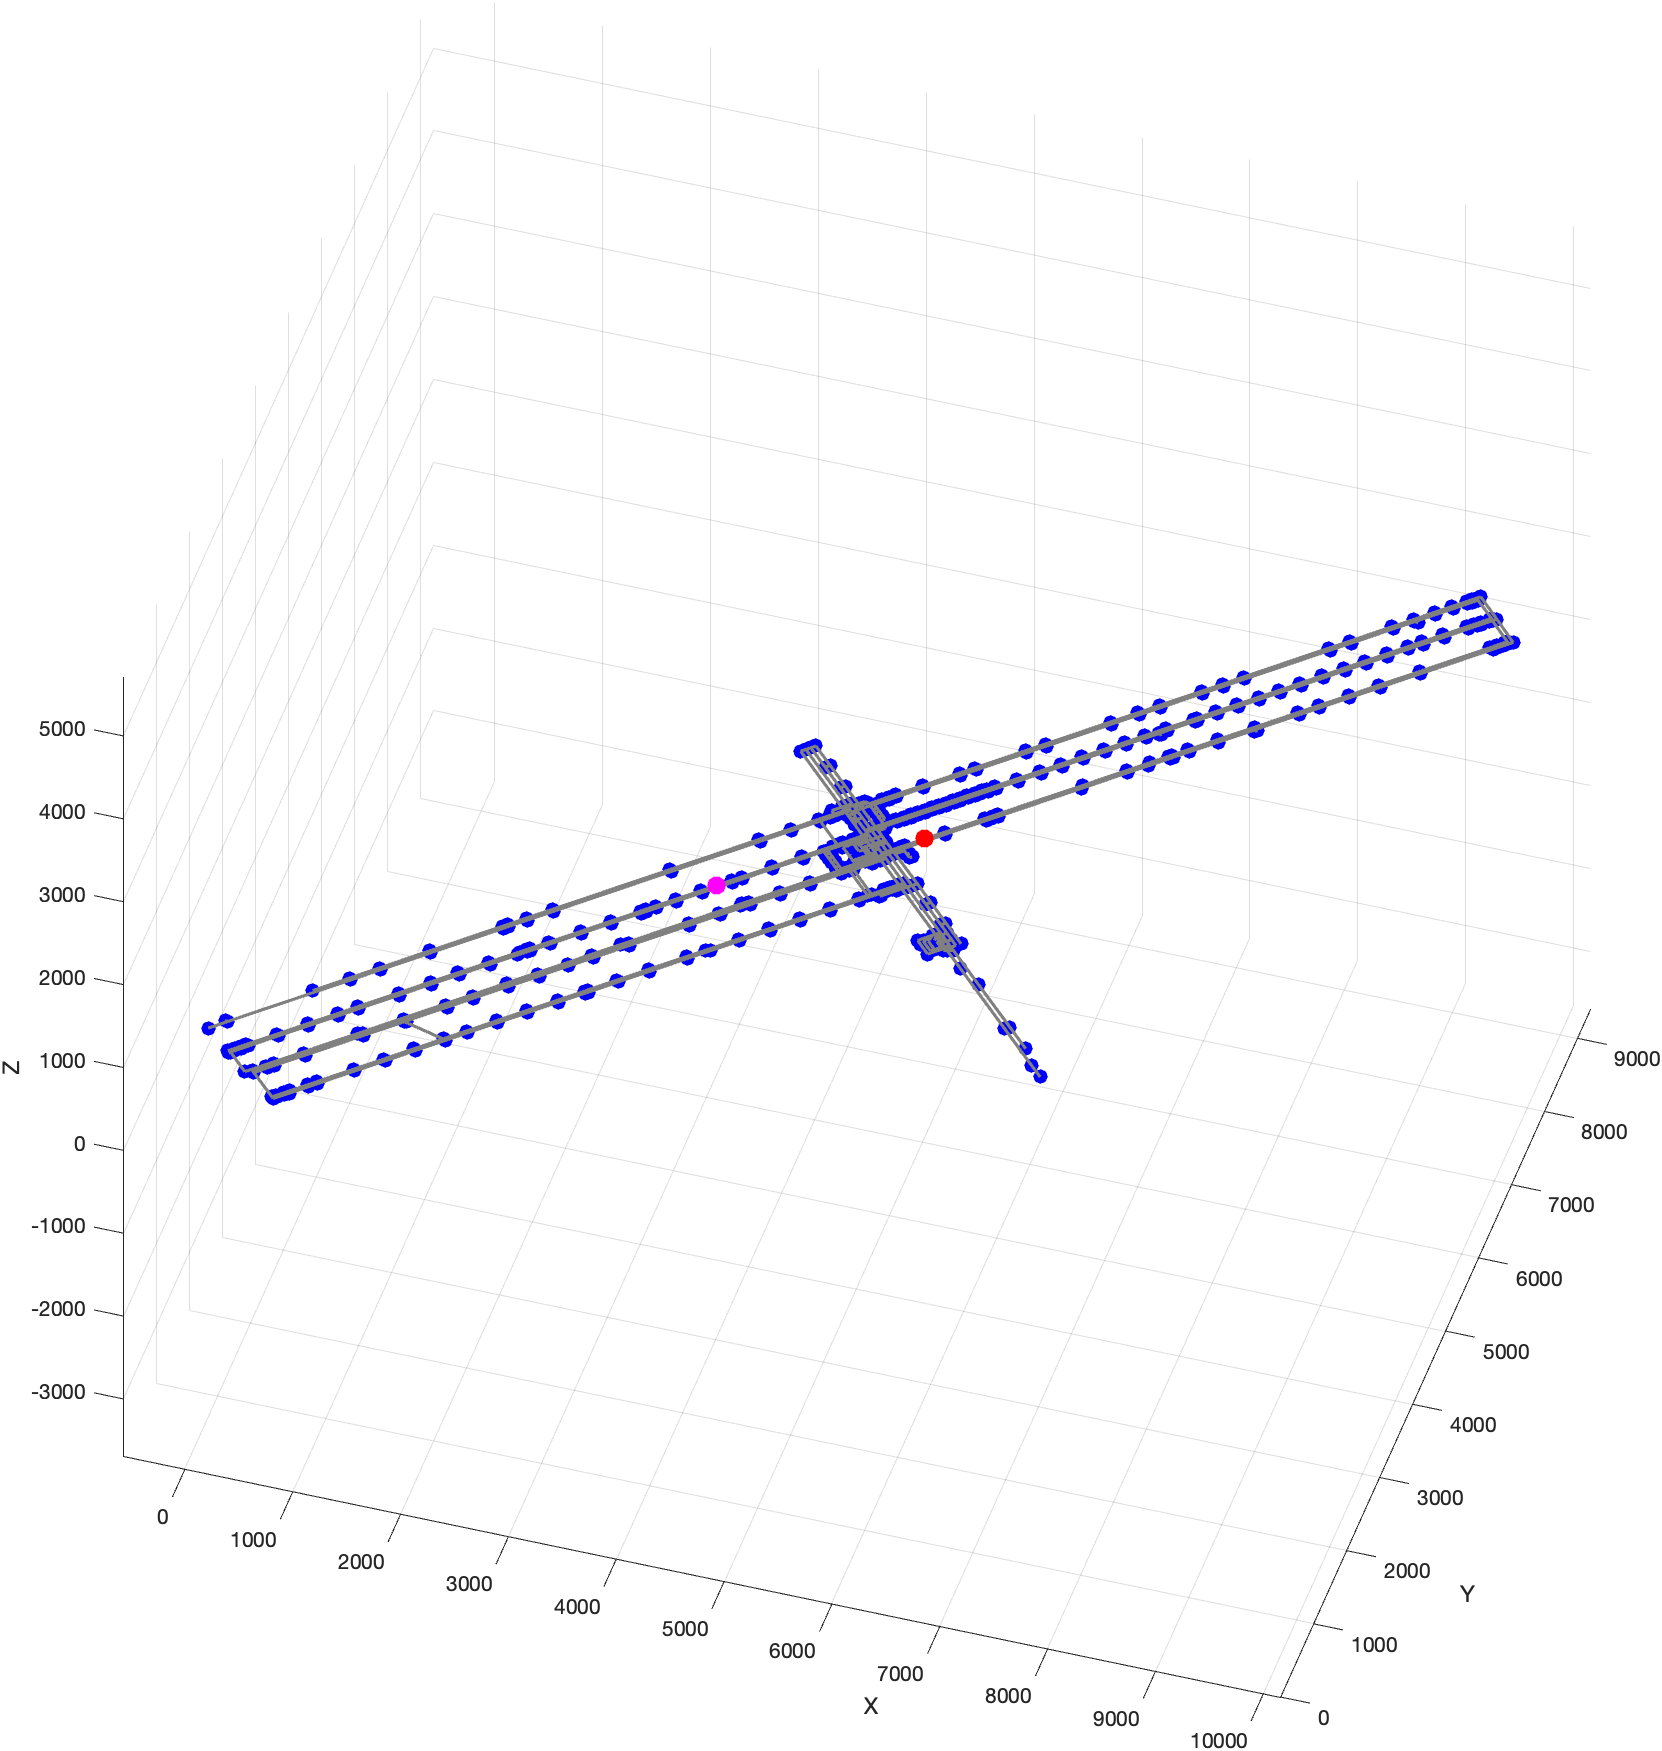
\includegraphics[width=\linewidth]{figures/fig13_att1_multi.png}
    \caption{3D view of the tunnel system with multiple inrush points, Attachment 1}
  \end{minipage}\hfill
  \begin{minipage}{0.48\textwidth}
    \centering
    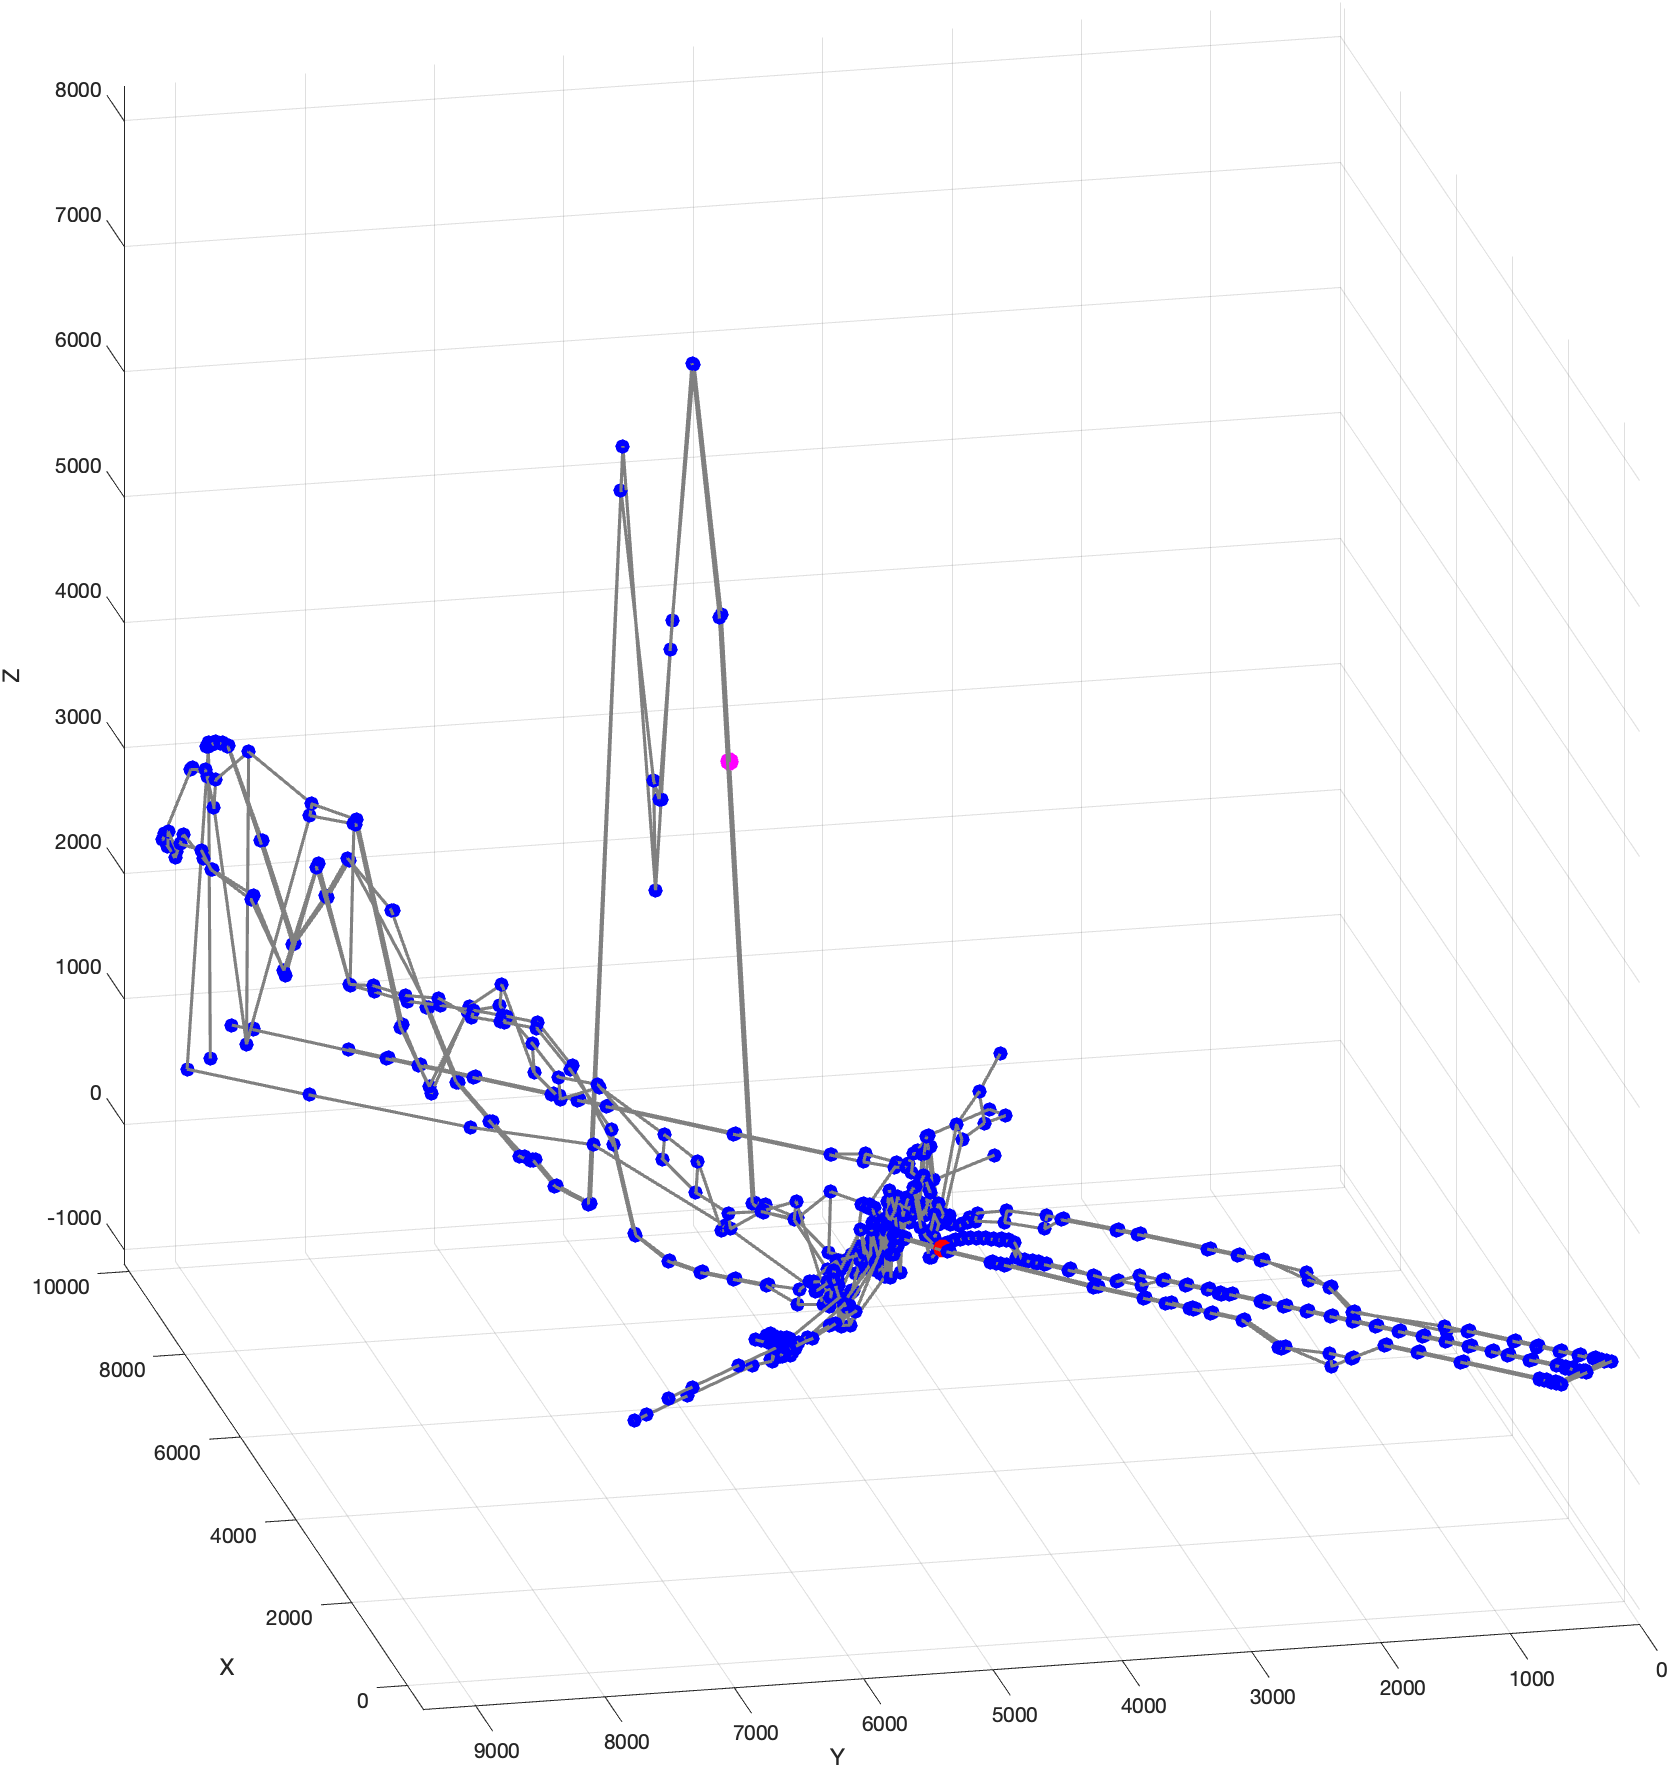
\includegraphics[width=\linewidth]{figures/fig14_att2_multi.png}
    \caption{3D view of the tunnel system with multiple inrush points, Attachment 2}
  \end{minipage}
\end{figure}

For Attachment 1, since all nodes are at the same height, the water spread from the new inrush point does not differ much from the previous one. As the figure shows, however, the new inrush point in Attachment 2 lies on an inclined tunnel, which makes the water spread more complex to account for. In addition, the coordinates and timing of the second inrush point are known in advance, so they can be treated as known quantities in the iterative simulation of the algorithm. The solution of Problem 3 follows the basic assumptions of Problem 1 for both attachments.

\subsubsection{Model and Solution}

The overall approach for Problem 3 is similar to Problem 1: both use a priority-queue algorithm to implement the abstracted inrush-spread model. The second inrush point added in Problem 3 increases the complexity and requires an extra delay mechanism to be implemented in code. In the program, this extra complexity shows up as an added delay setting and an improved flow algorithm, which ensures that water can flow uphill once the level and downhill tunnels are filled, in line with real-world behavior.

\subsection{Problem 4}

\subsubsection{Problem Analysis}

The approach to Problem 4 is similar to Problem 2: based on the inrush water-flow simulation from Problem 3 and the workers' initial positions, we perform dynamic scheduling to find the shortest time to reach any exit.

\subsubsection{Solution Approach}

From the delayed-inrush water-flow simulation in Problem 3, we obtain two vectors representing the times at which the inrush water reaches the nodes and floods the tunnels. Combined with the given delayed inrush rate and coordinates, these determine a worker's escape speed in a tunnel at any given global time, and give how the speed changes over time throughout the tunnel system. Following the solution code for Problem 2 and using similar constraints, we minimize the total escape time to complete the answer; this can be simulated and solved with Dijkstra's algorithm.

In Problem 4, the delayed second inrush may make the modeling more challenging. For this problem, however, the known time of the second inrush can be turned into given information, which converts it into the situation of Problem 2, so the optimization can be carried out in code.

\section{Model Testing and Analysis}

\subsection{Sensitivity Analysis}

When a parameter is being tested, all other parameters keep the values used in the calculations above. As Table~\ref{tab:sens} shows, the difference between the rate of change of each parameter and the rate of change of the corresponding dependent variable is within one order of magnitude, so the model is fairly robust. It is also reasonable that changing the downstream and upstream walking speeds leads to somewhat different final routes.

\begin{table}[htbp]
  \centering
  \renewcommand{\arraystretch}{1.35}
  \small
  \begin{tabular}{|>{\centering\arraybackslash}m{2.3cm}|>{\centering\arraybackslash}m{1.9cm}|>{\centering\arraybackslash}m{3.6cm}|>{\centering\arraybackslash}m{1.9cm}|>{\centering\arraybackslash}m{3.6cm}|}
    \hline
     & Parameter increase & Change in dependent variable & Parameter decrease & Change in dependent variable \\
    \hline
    Initial water height & 10\% & $t_{arrival}$ avg.\ $+4.8\%$ & 10\% & $t_{arrival}$ avg.\ $-4.8\%$ \\
    \cline{2-5}
     & 10\% & $t_{full}$ avg.\ $+1.7\%$ & 10\% & $t_{full}$ avg.\ $-1.6\%$ \\
    \hline
    Inrush flow rate & 10\% & $t_{arrival}$ avg.\ $+3.7\%$ & 10\% & $t_{arrival}$ avg.\ $-3.7\%$ \\
    \cline{2-5}
     & 10\% & $t_{full}$ avg.\ $+6.6\%$ & 10\% & $t_{full}$ avg.\ $+6.7\%$ \\
    \hline
    Downstream speed & 10\% & $Path$ elements changed $+31\%$ & 10\% & $Path$ elements changed $-31\%$ \\
    \hline
    Upstream speed & 10\% & $Path$ elements changed $+53\%$ & 10\% & $Path$ elements changed $-53\%$ \\
    \hline
  \end{tabular}
  \caption{Sensitivity analysis}
  \label{tab:sens}
\end{table}

\subsection{Reality Check}

For the simulated water spread, after checking the results against physics and everyday common sense, we found some extremely large values: for example, the water takes a very long time to reach some nodes and to fill some tunnels, even several years, which goes beyond common sense. Analyzing the cause, we may not have properly accounted for complex structures such as loops in the tunnel layout, leading to conflicting flow directions and other elements that are unreasonable under the basic assumptions. The program needs to be improved later to take these into account.

\subsection{Strengths and Weaknesses}

\subsubsection{Miner Escape Route Planning Model}

The model is built quite systematically: our team followed an overall coupled framework of water spread, network construction and route planning, and, starting from the results of the water-spread simulation, built a fairly complete emergency decision-making system. Next, we handled the problem dynamically in the modeling, paying attention to how the time-varying water flow affects the route weights and building the model on a time-dependent graph, which fits reality better. Finally, the model is highly adaptable: it can handle different tunnel systems as well as additional inrush points, so it extends well.

However, the model's basic assumptions are strong and involve many simplifications overall. For example, letting the water spread at a constant height of 0.1\,m ignores the continuity of the water flow and differs from real fluid behavior. Also, the model does not consider real-time data input or dynamic updating, so it lacks real-time capability; this needs to be improved in future work.

\section{Conclusions and Outlook}

This paper builds an effective model and proposes a coupled ``water-flow simulation -- network construction -- route optimization'' framework, which can effectively simulate the dynamic spread of water after a tunnel inrush and, on this basis, plan optimal escape routes for the miners. For the water spread, we computed the time series using a priority-queue algorithm, and took into account the effect of tunnel height differences on the flow direction, especially in Attachment 2, which allowed us to observe how and how strongly height differences matter. For the personnel escape, we converted the water-flow time series into a dynamic network with time-varying weights and, combined with Dijkstra's algorithm, carried out a time-dependent shortest-path search. This lets the miners tend to avoid flooded areas, with their routes gradually converging onto the main tunnel leading to the exit, which raises the chance of a successful escape. The model can be extended to scenarios with multiple inrush points, handling the complexity of multi-source inrushes through a delay mechanism and dynamic scheduling.

That said, our model simplifies the behavior of the water considerably (for example, a fixed initial spreading height of 0.1\,m and ignoring the continuity of the fluid), so a more realistic hydrodynamic model could be introduced in the future. Next, more constraints could be added to make the model more applicable to reality, taking more complex environmental factors into account, such as the miners' group behavior and physical limits. Finally, in future research we could introduce more efficient route-search algorithms, for example more efficient spatio-temporal graph algorithms, and combine them with parallel computing to handle larger tunnel systems.

\newpage
\section*{References}
\addcontentsline{toc}{section}{References}
\begin{enumerate}[label={[\arabic*]}, leftmargin=2.5em]
  \item Guo Zhixiong. A brief analysis of mine flooding problems [J]. \textit{Management \& Technology of SME} (First Ten-day Issue), 2012, (08): 156--157. (in Chinese)
  \item Williams, J. W. J. (1964). Algorithm 232: Heapsort. \textit{Communications of the ACM}, 7(6), 347--348.
  \item Dijkstra, E. W. (1959). A note on two problems in connexion with graphs. \textit{Numerische Mathematik}, 1(1), 269--271.
\end{enumerate}

\newpage
\noindent\textit{Note on the appendices:} the data-file names and Excel sheet names in the code are kept in Chinese because they must match the original competition data files: \texttt{{\cjkfont 附件}1.xlsx} / \texttt{{\cjkfont 附件}2.xlsx} are Attachment~1 / Attachment~2, and the sheets {\cjkfont 端点} and {\cjkfont 巷道} are the ``Endpoints'' and ``Tunnels'' sheets.

\appsection{A}{Problem 1 -- Solution Code for Attachment 1}
\lstinputlisting[style=py]{code/appA.txt}

\appsection{B}{Problem 1 -- Solution Code for Attachment 2}
\lstinputlisting[style=py]{code/appB.txt}

\appsection{C}{Problem 2 -- Optimal Route Algorithm Code}
\lstinputlisting[style=mat]{code/appC.txt}

\appsection{D}{Problem 3 -- Solution Code for Attachment 1}
\lstinputlisting[style=py]{code/appD.txt}

\appsection{E}{Problem 3 -- Solution Code for Attachment 2}
\lstinputlisting[style=py]{code/appE.txt}

\end{document}
